En este TP se lleva a cabo el análisis de distintas redes a partir de
la captura de paquetes, modelándolos de diversas formas utilizando
conceptos de la teoría de la información.
 
Un concepto importante en este contexto es el de \textit{información}. Sea $E$
un evento que ocurre con probabilidad $P(E)$. Decimos que al ocurrir
dicho evento hemos recibido

$$
I(E) = \log{\frac{1}{P(E)}}
$$
unidades de información.
 
Según la base del logaritmo usada sea $10$, $e$, o $2$, decimos que
hemos recibido Hartleys, nats, o bits.
 
Otro concepto importante es el de fuente de información con 
\textit{memoria nula}.
Una fuente de este tipo emite una secuencia de símbolos
provenientes de un alfabeto fijo de un tamaño finito $S
= \{s_1, \dots, s_n\}$, cada uno de los cuales tiene una probabilidad
de ocurrencia fija. Se dice que tiene "memoria nula" porque la
probabilidad de emitir un símbolo cualquiera es independiente de los
símbolos emitidos anteriormente.

Un concepto ligado una una fuente así definida es el de \textit{entropía}, que
es la suma de la información asociada a cada símbolo multiplicada por
su probabilidad; es decir:
$$
H(S) = \sum_{s \in S} P(s)I(s)
$$

Por último, una propiedad que vamos a tener en cuenta en nuestro
trabajo es que el valor máximo de la entropía (dada una fuente y
variando las probabilidades) es $log |S|$; valor que
alcanza cuando todos los símbolos son equiprobables.

\subsection{Frames Ethernet}

\begin{center}
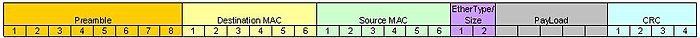
\includegraphics[scale=0.6]{Ether.jpg}
\end{center}

La imagen muestra los campos de un paquete de red Ethernet.
Uno de ellos es el EtherType,
que ayuda a saber qué tipo de protocolo está encapsulado dentro del paquete.
En este informe analizaremos distintos protocolos, pero entre ellos
nos enfocaremos con más detalle en el ARP.

\subsection{Protocolo ARP}

El protocolo ARP trabaja entre la capa de enlace y la capa de red. 
Es el encargado de mapear las direcciones IP de la red, de modo que estén asociadas con las direcciones MAC de los dispositivos de la red.
Los paquetes que usa el protocolo ARP pueden ser de tipo \textit{WHO-HAS} o de
tipo \textit{IS-AT}.

Los de tipo WHO-HAS son paquetes con destino MAC FF:FF:FF:FF:FF:FF (broadcast)
que se utilizan para pedir la dirección MAC del dispositivo con cierta
dirección IP.
Las de tipo IS-AT son respuestas de tipo unicast a paquetes WHO-HAS.
Estos contienen la dirección MAC pedida y al origen
del WHO-HAS que comenzó la comunicación como destino.

\begin{center}
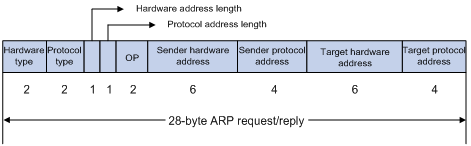
\includegraphics[scale=0.8]{arp.png}
\end{center}

Todo este intercambio de paquetes ayuda a armar la tabla de direcciones MAC e IP de los routers que forman parte de una red.
   
